\chapter{Event system}\label{section:events}
Events do not  Generally, events are reactions for some other actions. In software, actions can be divided into to categories:
\begin{description}
\item[HUMAN-TRIGGERED ACTIONS] \hfill \\
This type of actions represents natural notion of what events are. Mouse button clicks, keyboard key presses or perhaps cursor movements are human-triggered events. Each of them disposes certain properties, \eg mouse-click produces coordinates of click or key push produces the pressed character or perhaps set of characters if key sequence is used.
\item[APPLICATION-TRIGGERED ACTIONS]  \hfill \\
Are not triggered directly by application user. Typical application-triggered event is painting event which is responsible for drawing \fdocabbrevref{GUI} elements on the screen. User starts this event indirectly by manipulating application user interface.
\end{description}

Event is consequence of occurrence of certain action in running application. There are plenty of various types of events. Typical event might be key-press-event or perhaps mouse-click-event or repaint-gui-event.

Each\fdocinlinecode{cpp}{!}{QObject} subclass has ability to send events. Events are usually distributed by one entity which manages whole event process. This entity \enquote{sits} on the top of event loop. Event loop is part of application execution which encapsulates all events sent by objects inside the loop. Loop goes from time to time through all raised events from its underlying objects and delivers those events to target objects. Event loop structure looks similar to one in \autoref{listing:eventloop2}. Event loop exits if \enquote{exit} signal occurs.

Each Qt application has one main global event loop with\fdocinlinecode{cpp}{!}{QApplication} instance as managing entity (entity which caused the creation of the event loop). Consider \autoref{listing:eventloop}. Call on line \ref{listing:loop1} of \autoref{listing:eventloop} results in entering to global event loop, so that events from application objects, \eg from main application window, can be processed.


\begin{fdoccode}{cpp}{listing:eventloop}{Global event loop}
int main(int argc, char *argv[]) {
    QApplication a(argc, argv);
    
    // Display main application window here.
    .............

	// int QApplication::exec() triggers global event loop.
    return a.exec();(*@\label{listing:loop1}@*)
}
\end{fdoccode}

\begin{fdoccode}{cpp}{listing:eventloop2}{Typical event loop structure}
while() {
	if (exit) {
		return status;
	}
	check_queue_of_pending_events;
	process_all_pending_events;
	remove_processed_events_from_the_queue;
}
\end{fdoccode}

\begin{figure}[ht]
\centering
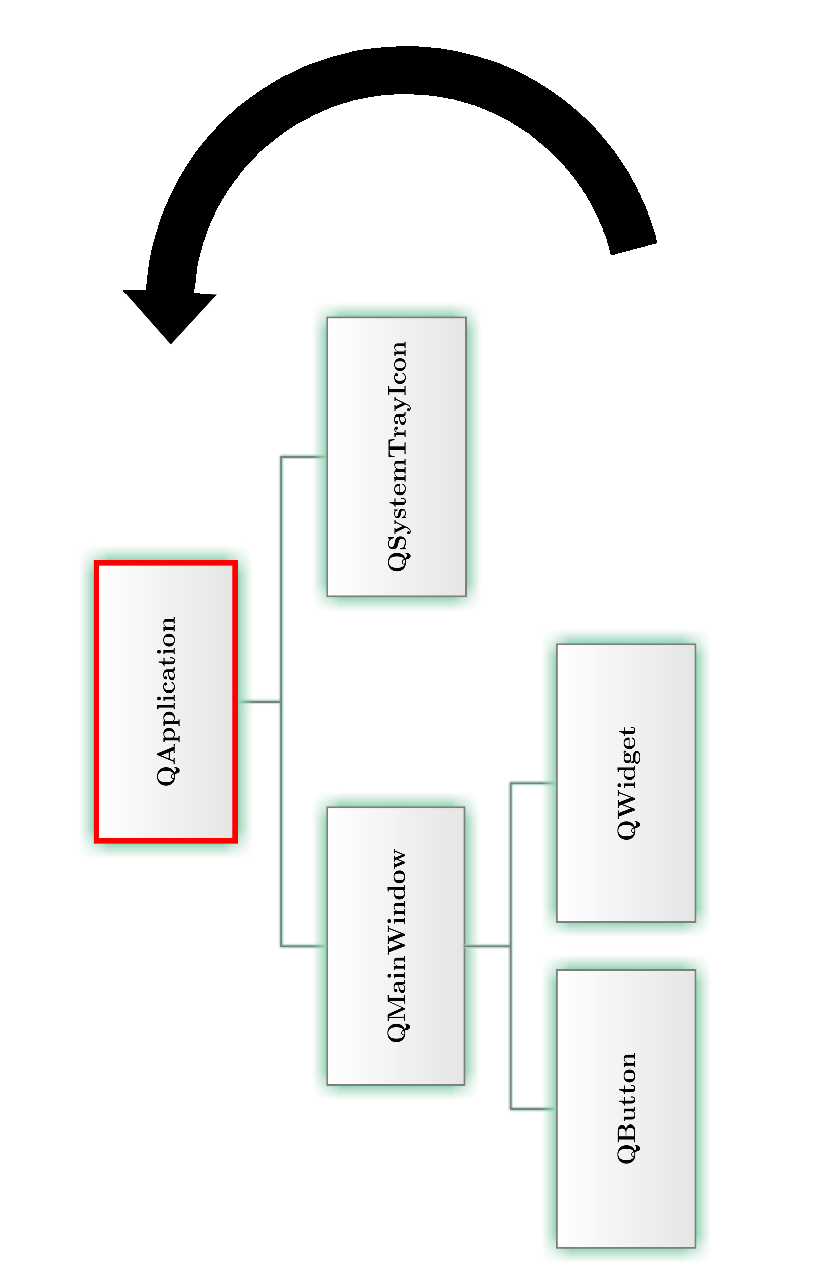
\includegraphics[angle=-90,width=11cm]{graphics/laboratory/15-eventloop.pdf}
\caption{Typical event loop}\label{figure:eventloop}
\end{figure}

Let's take a look at \autoref{figure:eventloop} which displays typical structure of Qt application.  Arrow indicates position of supervising entity (entity which triggered event loop). If\fdocinlinecode{cpp}{!}{QSystemTrayIcon} notices that certain event happened in it,\fdocinlinecode{cpp}{!}{QApplication} instance is notified about the situation and is given information about:
\begin{itemize}
\item type of event
\item event properties
\item sender
\end{itemize}
Event (object) is posted by\fdocinlinecode{cpp}{!}{QSystemTrayIcon} and appended to event loop queue for further processing and\fdocinlinecode{cpp}{!}{QSystemTrayIcon} possibly waits for backward event delivery from event loop.

\indent\fdocinlinecode{cpp}{!}{QApplication} event loop iterates and finds new unsolved events which are eventually removed from the queue and sent to their senders.\fdocinlinecode{cpp}{!}{QSystemTrayIcon} then \textit{handles} the event and responds with expected behavior which finally concludes life of this event.

Handling event means calling \textit{event handler} -- some kind of special method. If you handle some events in one object, sometimes you need to \textit{propagate} the same event in another object too. For example if you move use\fdocinlinecode{cpp}{!}{QButton} (ordinary button) instance by mouse, then paint-event is raised, because\fdocinlinecode{cpp}{!}{QButton} needs to be repainted on the screen, and this event is propagated to parent object which is usually application window which needs to redraw itself too. Some events are propagated and other ones are not.

Easiest way to handle events in Qt is reimplementing available event handlers. Each\fdocinlinecode{cpp}{!}{QObject} offers specific handlers. All handlers are declared as protected methods. See \autoref{listing:reimplm} (example\fdocinlinecode{text}{!}{sources/laboratory/12-child-event}) for typical extension of event handler. In this case, we reimplemented behavior of child-event which is triggered if child is added or removed to particular\fdocinlinecode{cpp}{!}{QObject} instance. Event handler of superclass is called on line \ref{listing:handl} because we want to only extend the original handler and not to replace its behavior completely. This approach is common in Qt and is used especially for \fdocabbrevref{GUI}-related events.

\begin{fdoccode}{cpp}{listing:reimplm}{Reimplementing event handler}
// myqobject.h
class MyQObject : public QObject{
	Q_OBJECT

    public:
		explicit MyQObject(QObject *parent = 0);

    protected:
		void childEvent(QChildEvent *event);
};

// myqobject.cpp
#include <QChildEvent>

#include "myqobject.h"


MyQObject::MyQObject(QObject *parent) : QObject(parent) {
}

void MyQObject::childEvent(QChildEvent *event) {
    if (event->added()) {
		qDebug("Child %s (%s) was added to %s.",
	       	event->child()->metaObject()->className(),
	       	qPrintable(event->child()->objectName()),
	       	qPrintable(objectName()));
    }
    else if (event->removed()) {
		qDebug("Child %s (%s) was removed from %s.",
	       	event->child()->metaObject()->className(),
	       	qPrintable(event->child()->objectName()),
	       	qPrintable(objectName()));
    }

    QObject::childEvent(event);(*@\label{listing:handl}@*)
}
\end{fdoccode}

% TODO: 
% metoda QObject::startTimer...událost dále customEvent
% diagram cyklu
% deleteLater vs delete
% qapplication event loop

\section{Event filters}
Classic event handlers maybe unusable if you want to handle all events in one place. One solution is to use generic\fdocinlinecode{cpp}{!}{bool QObject::event(QEvent * e)} event handler which catches all events. Another solution of this approach is event filtering. Event filter is ordinary method which accepts destination\fdocinlinecode{cpp}{!}{QObject} instance and event object. Example (\autoref{listing:reimplm2}) shows the approach quite clearly.

\begin{fdoccode}{cpp}{listing:reimplm2}{Using event filter}
// myqobject.h
class MyQObject : public QObject {
	Q_OBJECT

    public:
		explicit MyQObject(QObject *parent = 0);

    protected:
		bool eventFilter(QObject *object, QEvent *event);
};

// myqobject.cpp
#include <QEvent>

#include "myqobject.h"


MyQObject::MyQObject(QObject *parent) : QObject(parent) {
    installEventFilter(this);
}

bool MyQObject::eventFilter(QObject *object, QEvent *event) {
    qDebug("Event happened in %s.", qPrintable(object->objectName()));

    if (event->type() == QEvent::ChildAdded) {
	qDebug("Observing child-event for %s and child %s.",
	       qPrintable(object->objectName()),
	       qPrintable(static_cast<QChildEvent*>(event)->child()->objectName()));
    }

    return QObject::eventFilter(object, event);
}
\end{fdoccode}


% TODO: Custom events.
%\subsection{Custom events}

% TODO: QObject timers
%\subsection{QObject timers}